\documentclass[11pt]{article} 

% Preamble section
\newcommand{\bs}{\ensuremath{\backslash}} % Alias para backslash
\usepackage[utf8]{inputenc}
\usepackage[spanish]{babel}
\usepackage{graphicx}
\newcommand{\HRule}{\rule{\linewidth}{0.5mm}}


\title{Muphic: Composición Musical Automática basada en Imágenes} % Título tentativo
\author{Johan Bertrand \and Carlos Catalán \and Vladimir Giorgiev}
% \date{7 de Mayo de 2012}


\begin{document}


\begin{titlepage}
\thispagestyle{empty}

\begin{center}


% Upper part of the page

\includegraphics[width=0.3\textwidth]{./graphics/escudo-ucm.png}\\[1cm]    

\textsc{\LARGE Universidad Complutense de Madrid}\\[1.5cm]

\textsc{\Large Proyecto fin de carrera}\\[0.5cm]


% Title
\HRule \\[0.4cm]
{ \huge \bfseries Muphic: Composición Musical Automática basada en Imágenes}\\[0.4cm]

\HRule \\[1.5cm]

% Author and supervisor
\begin{minipage}{0.4\textwidth}
\begin{flushleft} \large
\emph{Authors:}\\
Johan \textsc{Bertrand}\\
Carlos \textsc{Catalán}\\
Vladimir \textsc{Georgiev}
\end{flushleft}
\end{minipage}
\begin{minipage}{0.4\textwidth}
\begin{flushright} \large
\emph{Supervisor:} \\
Jaime \textsc{Sánchez}
\end{flushright}
\end{minipage}

\vfill

% Bottom of the page
{\large \today}

\end{center}

\end{titlepage}

\chapter*{Prefacio}
\addcontentsline{toc}{chapter}{Prefacio}
\todo{reorganizar todo lo que está antes del índice para que quede acorde a lo especificado}
\phantomsection
\chapter*{Tags}
\todo{Pendiente de hacer}
\newpage

\phantomsection
\chapter*{Firmas}
\todo{Pendiente de hacer}
\chapter*{Agradecimientos}
\addcontentsline{toc}{chapter}{Agradecimientos}
% 6
\tableofcontents
\newpage
\chapter{Introducción}

\torev{Última revisión hecha el 11-06-2012}\\

	\section{¿Qué es Muphic?}
	
		\vspace{0.2in}
		Muphic es un software capaz de producir piezas musicales compuestas automáticamente a partir de una imagen. Es el resultado de un proyecto de sistemas informáticos comenzado en octubre del 2011 por 3 alumnos de Ingeniería Informática, cuyo propósito es generar música a partir de imágenes basándose en el fenómeno de la sinestesia.\\
		
		Antes de proceder a describir el proyecto, es necesario explicar qué es la sinestesia, un término de gran importancia a lo largo del documento. Tal y como afirman Ramachandran y Hubbard en \cite[pg.~4]{paperSyn}:
		
		\begin{quote}
		\emph{``La Sinestesia es una curiosa condición según la cual un individuo de cualquier otra manera normal experimenta sensaciones en una modalidad cuando una segunda modalidad es estimulada. Por ejemplo, un sinésteta puede experimentar un color determinado siempre que se encuentre con un tono particular(p. ej., C\# puede ser azul) o puede ver un número dado tintado siempre de un cierto color (p. ej., ‘5’ puede ser verde y ‘6’ puede ser rojo).''}
		\end{quote}
		
		Dentro de la sinestesia, nos centraremos en la sinestesia auditivo-visual (aquella que relaciona los sentidos del oído y la vista), y más concretamente en la estimulación del sentido auditivo a partir de una percepción visual. Estudiaremos cómo reproducir esa asociación neurológica de las sensaciones visuales con los fragmentos musicales para poder generar composiciones musicales.\\
		 
		
		De forma resumida, dado que se entrará en detalle en secciones siguientes, la aplicación desarrollada analiza una imagen de entrada y utiliza el contenido de dicho análisis para generar una pieza musical mediante algoritmos de composición automática.\\

\color{blue}
		Este proyecto por tanto se puede dividir en dos fases críticas:
		%Este proyecto trata por tanto 2 temas distintos:
\color{black}
		
		\begin{itemize}
		
		\item Análisis de imágenes: la imagen de entrada se debe procesar y estudiar hasta obtener la información deseada (formas, colores, tamaños, ...).

		\item Composición algorítmica: Con la información obtenida a partir de la imagen y el conocimiento de cómo se relaciona con la música, se pasa a componer, de forma automática, todas las partes que \color{blue}forman \color{black} nuestra pieza musical: ritmo, melodía y armonía.
		\end{itemize}
		
		\color{blue}El segundo punto va a depender enormemente del primero, con distintos análisis de imagen se obtiene pequeñas diferencias en las descripciones de las imágenes de entrada. Y por tanto las composiciones musicales serán parcialmente diferentes, ya que la información procesada por el compositor será distinta en cada caso. Además, la elección de los algoritmos de composición cambiarán de forma significativa la pieza musical final.\\\color{black}
		
		En el desarrollo de este proyecto hay ciertos aspectos importantes que se ha considerado y es necesario mencionar:	

		\begin{itemize}
		
		\item \emph{La base de la correlación audio-musical será la sinestesia}:
			\vspace{0.1in}
			\\La sinestesia, como ya se ha comentado, es la pieza clave en la creación de música basada en imágenes (ver Sección~\ref{subsubsec:estudioSinestesia}) frente a otras alternativas de planteamiento.\\
			Entre estas alternativas, cabe destacar la reacción psicológica sociocultural del cerebro humano ante la música y los colores. Es decir, estudios muestran que el verde, el azul y otros colores con \color{blue}longitudes \color{black} de onda bajas se relacionan con la calma, mientras que colores con longitudes de onda altas aumentan el nerviosismo y la inestabilidad (\cite{colorpsy}). Hay, por otro lado, multitud de investigaciones sobre la psicología de la música y su relación con distintas emociones y sensaciones, como las asociaciones entre los modos griegos y los estados de ánimo (\cite{micrologus}). Una posible rama de desarrollo procedería juntando ambos ámbitos, la psicología del color y la de la música, para generar la música deseada en función de la imagen dada.\\
		\item \emph{No se tienen en cuenta objetos físicos}:
			\vspace{0.1in}
			\\El objetivo del análisis no es tanto obtener información de qué es lo que la imagen representa (reconocimiento e interpretación), sino los colores y formas que contiene, y su distribución y características dentro de la misma (segmentación y descripción). \color{blue}Es decir, si tenemos una imagen con un elefante no queremos reconocer el ``elefante'' sino que hay una figura  redondeada con una parte alargada (la trompa) y que tiene un colo azul grisáceo y se encuentra en el centro de la imagen.\color{black}
		\item \emph{La imagen es estática}:
			\vspace{0.1in}
			\\Se consideran para el análisis formatos de imagen estática (tales como bmp, jpg o png), y no animada (vídeo o archivos de animación). Este planteamiento condiciona el proceso de correlación imagen-música, ya que se pretende obtener una salida no estática, como es la música, a partir de una imagen inmóvil. Veremos más adelante cómo se obtiene ese efecto de \emph{dinamismo} a partir de la información proporcionada por una imagen.
		\item \emph{Generación de contenido frente a acoplamiento de creaciones preestablecidas}:
			\vspace{0.1in}
			\color{blue}\\Es importante recalcar que en el proceso de composición las piezas generadas se construyen desde cero y no parten de ninguna estructura predefinida. No se usarán por tanto piezas ya compuestas o estructuras conocidas como ``ladrillos'' para construir una pieza nueva, como una base de datos o adaptaciones de piezas musicales enteras. Es cierto que se pueden seleccionar ciertos parámetros de la composición pero sirven para matizar las composiciones (tempo, instrumentos, ...). \color{black}
		\end{itemize}
		
		Además, resulta importante resaltar que siendo el objetivo final del proyecto generar música no se ha buscado que compita con obras de grandes compositores. Nuestro modelo es la creación de la llamada música de ambiente; es decir, música que, siendo voluntariamente no atrayente ni excesivamente interesante, tiene como requisito principal el no ser molesta. Se sigue por tanto la línea de la música mostrada por Brian Eno en \emph{Música para Aeropuertos (1978)}:
		
		\begin{quote}
		\emph{``[La música ambiente es] Algo de lo que puedes entrar o salir discretamente. Puedes atender o puedes elegir no distraerte con ella si quisieras hacer algo mientras la música está reproduciéndose.''}, (\cite{BrianEnoInterview}, entrevista con Brian Eno).
		\end{quote}		
		
		Por último, se ha de \color{blue}añadir \color{black} que el ámbito de la composición basada en imágenes es uno muy estudiado pero a la vez poco desarrollado. Es decir, aunque existe una gran cantidad de estudios sobre la sinestesia y la composición musical automática (como se puede ver en la Sección~\ref{sec:estadodelarte}), aún quedan muchas cuestiones que investigar y áreas que profundizar \color{blue}así como la conexión entre la música y la imagen.\\ \color{black}
		
		\color{blue}Teniendo todo eso en cuenta, comentaremos en las siguientes secciones cómo se ha abordado el proceso. En primer lugar hablaremos del estado del arte y las diferentes investigaciones y pruebas realizadas hasta el momento. Seguidamente se expone la forma de usar la herramienta que se ha desarrollado. Más adelante, en la tercera sección, exponemos de forma detallada los algoritmos usados tanto en el análisis de imagen como en la composición musical. Por último se explica el sistema en detalle y cómo se ha realizado. \color{black}
		

\section{Motivación}


La principal motivación de este proyecto nace, por supuesto, del interés de los participantes en la música y su aplicación en el área de la computación. Aunque existe una lista interminable de aplicaciones orientadas a esa relación música-informática (como puede ser SunVox \cite{SunVox} en el ámbito de los sintetizadores musicales, o la famosa aplicación ToneMatrix \cite{toneMatrix}, por citar dos ejemplos), el interés de este proyecto parte de un área en particular: la composición algorítmica.\\

El campo de la composición algorítmica consta de muchos estudios y trabajos realizados sobre la materia. Sin embargo, gan parte de ellas caen dentro de dos casos: o bien se basan en el acoplamiento y unión de diferentes piezas previamente compuestas aplicándoles ciertas modificaciones (consiguiendo resultados auditivamente agradables, pero en ningún momento ``nuevos''), o bien busca una creación completa de la melodía. Como ya se comentó en la sección anterior, es este último campo el que motiva el desarrollo de este proyecto. Se busca por tanto la composición genuína de piezas musicales, útil como fuente de inspiración para usuarios compositores o la generación de música de ambiente.\\

Dentro de la composición algorítmica, el interés de los intregrantes del proyecto se centra sobre todo en dos aspectos fundamentales:

\begin{itemize}

	\item De todas las formas posibles de generación de música algoritmica existentes, se tiene especial interés en una generación determinista. Esto es, en vez de partir de algortimos genéticos o cualquier otro tipo de diseño basado en un entrada aleatoria, se desea obtener una pieza musical que suponga la representación de un objeto constante y perteneciente a conexto no auditivo. Es esta búsqueda la que lleva a plantearse el usar imagenes como entradas a estos algoritmos.
	
	\item Además, dado que se tiene una entrada gráfica al algoritmo, la interpretación de la misma no esté sujeta a concepciones, ya sean culturales o personales, de nosotros que diseñamos los algoritmos de composición. Buscando cumplir este objetivo es donde nos encuentramos con la sinestesia, fenómeno que relaciona diferentes sentidos que además está siendo fuertemente estudiada por la rama de la psicología.
	
\end{itemize}

Se relacionan así dos elementos que incitan gran interés en la comunidad científica y que, si bien han sido estudiados por separado (como bien se aprecia en la siguiente sección), juntos componen un objeto de estudio apenas observado. Es la motivación de este proyecto el estudiar y experimentar en este ámbito, con el objetivo de expandir su trasfondo académico y observar las posibilidades que ofrece.\\

Cabe destacar también la inclinación a crear una aplicación de esta índole para dispositivos móviles. Una versión simple y accesible de este sistema puede ser de gran interés en este mercado, ya que las entradas gráficas se pueden obtener con gran facilidad gracias a las cámaras integradas en la mayoría de las plataformas portátiles. También se facilita enormemente el proceso de testeo de los diferentes resultados permitiendo su rápido progreso.
\section{Estado del Arte}
\label{sec:estadodelarte}

\subsection{Estudio sobre Sinestesia}
\label{subsubsec:estudioSinestesia}

\todo{
Esquema:
\begin{itemize}
\item introducción sinestesia color-música
\item los primeros que asociaron color con sonido
\item una aproximación a través de la psicología
\item experimentos y cosas hechas sobre la sinestesia (sin técnicas de composición)
\end{itemize}
}


Dentro de la sinestesia, la parte que es importante en este proyecto es la llamada sinestesia musical. Esta consiste en mezclar la experiencia auditiva con la visual. Se ha estudiado este tipo de sinestesia porque cabe pensar que sería una fuente de información razonable para poder empezar a realizar la conversión de imagen a música.
Según el neurocientífico David Eagleman, las personas de forma innata tienen la tendencia de conectar sentidos, entre otros visual y auditivo (sonidos con formas y sonidos con colores, como se ve en \cite{VideoRedesFliparColores}).\\

Varios artistas y científicos en el tiempo han expresado su capacidad sinestésica a través de sus obras o documentando y experimentando con este fenómeno. Desde la antigua Grecia se intentaba encontrar esa equivalencia entre los colores y los sonidos. Aristóteles en su ensayo (De Sensu et Sensato \cite{DeSensuEtSensato}, 439b30) realiza una descripción de los colores comparándolos directamente con la armonía presente en la música. Siguiendo esa línea científica-filosófica, Newton asignó un color a cada nota de la escala diatónica siguiendo los colores de su prisma de C (Do) rojo a B (Si) violeta.\\

Otra aproximación a la relación música-imagen que normalmente siguen los artistas es a través de la experiencia con el fenómeno de la sinestesia. Encontramos entre ellos al compositor Scriabin, quien hizo una asociación entre los colores y los acordes que aparecen en música usando el círculo de quintas. Kandinsky, otro artista como Scriabin pero pintor, partiendo de la pintura ha investigado y defendido fervientemente la posibilidad de asociar la música a la pintura y su relación directa (\cite{ConcerningSpiritualArt}). Resalta aspectos como por ejemplo que la escala de intensidad de los sonidos estaba relacionada con la intensidad de los trazos de la pintura, también distingue timbres de instrumentos por colores asignando a cada familia colores parecidos.\\

Las investigaciones llevadas a cabo por el psicólogo Köhler en 1929 (\cite{GestaltPsychology}) y las hechas recientemente demuestran que tenemos una conexión profunda entre los sonidos y formas, además de los colores. Marks, en \emph{The Unity of the Senses} (\cite{TheUnityOfTheSenses}) encuentra una asociación entre los tiempos en música y las formas, tal que cuanto más angular e irregular es una figura el tempo o las notas son más rápidas.También declara sobre los colores que:
\begin{quote}
\emph{``Por desgracia, al final uno descubre que no hay una asociación sinestésica entre notas musicales y colores que prevalezca ante las demás''}.\\
\end{quote}

Después de ver la aproximación a través de la experiencia (con los trabajos de Aristótles, Scriabin o Kardinsky ya mencionados) a través de la lógica o fundamentación matemática (como los propuestos por Newton o Köhler), queda claro que cada persona sinestésica es única y puede haber grandes diferencias entre unas experiencias sinestésicas y otras. Es por tanto importante poder encontrar asociaciones aceptables y ponerlas en práctica para comprobar los distintos resultados.

\subsection{Composición basada en imagenes}

\torev{Última revisión realizada: 20-06-2012}\\

Para poder componer música a partir de datos gráficos necesitamos crear una correlación entre los elementos que tenemos en la parte gráfica y en la parte musical. Esta correspondencia no es fácil de conseguir, y a través de la historia se han desarrollado varias teorías que se han llegado a poner en práctica. Los primeros intentos de síntesis fueron los instrumentos llamados ``órganos de color'' que acompañaban al sonido con una muestra visual.

El primer instrumento lo construyó Louis Bertrand Castel (1730), se trataba de un clavecín al que se le había incorporado una pantalla y un sistema de iluminación. Cuando se pulsaban las teclas se iluminaban los colores correspondientes en la pantalla \cite{organosColor}. A este experimento le continuaron muchos otros que incorporaban mejoras, pero al ser una correspondencia muy directa entre nota y color, al final se obtiene poca diversidad. Además es una correspondencia de la música a la estimulación visual mientras que nuestro interés se centra en la otra dirección, de la imagen a la música.\\

Desde hace unas décadas, gracias a los avances tecnológicos, se han investigado activamente los algoritmos automáticos de composición. Una posible clasificación de los diferentes algoritmos basada en su característica principal sería: modelos matemáticos, sistemas basados en conocimiento, gramáticas, evolutivos, sistemas con aprendizaje e híbridos \cite{AIMethodsForComposition}. \\

\color{blue}
\begin{itemize}
	\item Modelos matemáticos: los más usados son los procesos basados en sistemas estocásticos y cadenas de Markov. Como ejemplo significativo de estos modelos destaca Cybernetic Composer \cite{AIMusicSurvey}. Otra subcorriente son los basados en la teoría del caos \cite{ChaosTeoriaMusica}.
	\item Sistemas basados en conocimiento: dependiendo de cómo se represente el conocimiento y cómo se manipula podemos hacer diferentes clasificaciones. Como ejemplos relevantes se tienen CHORAL \cite{HistoryAlgorithmicComp} o SICOM \cite{SICOM}.
	\item Gramáticas: fueron las primeras técnicas usadas. Se suelen mezclar con técnicas probabilísticas obteniendo gramáticas indeterministas, ya que si no, puede producirse música poco variada. Destacan el proyecto EMI \cite{HistoryAlgorithmicComp} o Steedman y su generador de música Jazz \cite{AIMethodsForComposition}.
	\item Algoritmos evolutivos: se dividen en dos posibilidades según la función de evaluación. La primera es usando una función de evaluación automática. Como ejemplo se tiene McIntyre \cite{AIMethodsForComposition}. La otra posibilidad es usar una evaluación humana, que es bastante más lenta y además ambigua. La herramienta de improvisación de Jazz de Biles, GenJam \cite{GenJam}, es un ejemplo importante de este tipo.
	\item Sistemas con aprendizaje: están abiertas varias líneas de investigación según las diferentes formas del proceso de aprendizaje (adquisición de conocimiento del sistema). Una posibilidad es través de redes neuronales artificiales, un ejemplo significativo es EBM \cite{AIMethodsForComposition}. Otra manera es con aprendizaje automático (aprendizaje máquina) donde destaca el ejemplo de MUSE \cite{AIMethodsForComposition}.
	\item Híbridos: intentan combinar lo mejor que ofrecen los diferentes sistemas posibles, un ejemplo relevante es HARMONET \cite{AIMethodsForComposition} que combina sistemas con aprendizaje (redes neuronales) con sistemas basados en conocimiento.\\
\end{itemize}
\color{black}

Pero no solo la algoritmia es variada, también podemos clasificarla de diferente forma según el tipo de música que se quiera componer: micro-composición (diseño de sonidos) y la macro-composición (combinación de sonidos ya diseñados para la creación de una obra musical) \cite{AudioVisualSurvey}. En nuestro caso nos interesan los algoritmos de macro-composición basados en el fenómeno de la sinestesia.\\ 

Hay varias aproximaciones de compositores basados en imagen , algunos de ellos como Phonogramme \cite{ImageBaseComposition} \cite{Phonogramme} consisten en un editor gráfico que interpreta la imagen como una partitura. La imagen representa la relación bidimensional de tonos y duración de los sonidos, es decir, la imagen es una partitura que se lee de izquierda a derecha en el tiempo y de abajo a arriba en la altura de los tonos. 
\\El problema de este algoritmo desde el punto de vista de la sinestesia es que las imágenes son partituras y deben estar diseñadas para ser usadas con este fin (usando el editor gráfico), no acepta cualquier entrada gráfica. Esta línea de investigación se hace valer de la consexión psicológica que tenemos entre formas y sonidos, pero realmente no busca la sinestesia como base.\\

Otra opción es la propuesta basada en el concepto de ``croma'' (o índice de cromatismo) \cite{bricksConvertsMusic}. Se subdivide la imagen en bloques (ladrillos cromáticos) los cuales tienen un índice de cromatismo, esto sirve para generar o asignar trozos de música que pueden ser cogidos de una base de datos o ser creados por un experto (compositor). Al no haber una correspondencia directa entre la imagen y la música, este proyecto no está fundamentado en la sinestesia. Si bien recoge algunas ideas más adelante pierde la esencia de la sinestesia.\\

También destacamos el trabajo realizado por Xiaoying Wu y Ze-Nian Li \cite{ImageBaseComposition} en el que se analiza la imagen en tres pasos. Primero: hacer una \emph{Partición} de la imagen en piezas (divisiones, trozos) más pequeñas. Segundo: realizar la \emph{Secuenciación} de esas piezas para darles un orden en el tiempo. Tercero: aplicar un \emph{Mapeado} de las piezas de imagen a notas musicales.
\\Al ser una correspondencia directa entre la imagen y la música, este trabajo sigue parcialmente la sinestesia y la psicología de las formas y colores aunque este no es su propósito final.\\ 

\color{blue}De forma adicional, cabe mencionar dos trabajos interesantes en un ámbito menos académico.
El primero es un trabajo realizado por un equipo ruso \cite{dibujosymusica}, que permite hacer un dibujo simple (compuesto por un único trazo) y observar cómo se transforma en una melodía distinta dependiendo del trazo realizado y la herramienta con la que se ha realizado. Aunque parte de una base musical estática, a la que van ``maquillando'' de distintas formas dependiendo de la entrada gráfica, es digno de mención su facilidad de uso y la calidad de los resultados obtenidos.\\

El segundo de ellos es el realizado por el físico Lauri Gröhn \cite{rusofotos}, que aplica una serie de reglas basadas en la sinestesia para realizar composiciones algorítmicas postprocesadas. Basa el análisis en un estudio por secciones de la figura de entrada, mediante el cual va generando pequeñas porciones musicales a medida que recorre distintas regiones de la imagen divididas previamente de forma uniforme.\\\color{black}

Por último destacamos el trabajo de A. Pintado \cite{portutesis} en el que hace una investigación de la sinestesia y la percepción de las formas para poder generar ritmos. Analizando una imagen de entrada obtiene sus formas y líneas los cuales traduce a ritmos que genera usando  una relación directa entre el ritmo y la inestabilidad de las figuras. Este trabajo se centra en la línea de la sinestesia, especialmente en las formas de las figuras y los ritmos musicales, dejando de lado los colores y los tonos musicales. Por tanto ha sido una buena fuente de información aunque trate sólo parcialmente nuestro objetivo.\\ 

Todos estos algoritmos tienen en común un problema implícito puesto que dada una imagen cada persona espera una correspondencia musical diferente. Por tanto es difícil determinar el fitness o validez de cada algoritmo sabiendo además que la entrada gráfica puede tener infinidad de interpretaciones de todos sus valores disponibles.



\section{Algoritmos de Composición}
\label{sec:algcomp}
\section{Sistema}

morralla

\section{Guía de Uso}

	\subsection{Introducción}
		
		Esta sección pretende mostrar una vista general de la aplicación y sus opciones. A lo largo de ellan se explicarán todos los módulos del programa con los que el usuario tiene contacto y detallará la función de determinados mecanismos.\\
		
		\begin{figure}[htbp]
		\centering
		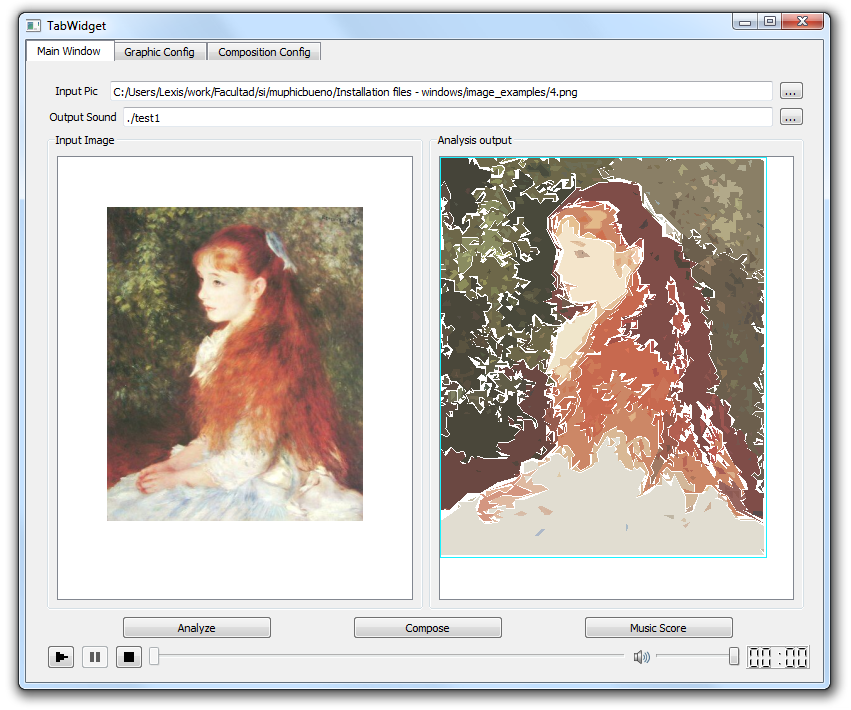
\includegraphics[scale=0.57]{graphics/interfazoverview.png}
		\caption{Vista general de la aplicación}
		\label{fig:interfazoverview}
		\end{figure}
		
		Como vemos en la Figura~\ref{fig:interfazoverview}, la aplicación dispone de 3 pestañas: Main Window, Graphic Config y Composition Config. La primera dispone de toda la funcionalidad necesaria para lanzar la aplicación, mientras que las otras 2 aportan opciones para configurar el comportamiento del análisis y la composición.\\
		
		De forma general, todo usuario, experto o inexperto, se puede valer de la primera pestaña para usar la composición. Sin embargo, un usuario avanzado con conocimientos musicales y de qué tipos de análisis gráficos se realizan puede navegar por las pestañas restantes para configurar el completo proceso mediante los parámetros ofrecidos.
		
		Se procede por tanto a explicar cada pestaña una por una.

		\subsubsection{Ventana principal}
		
		Se encarga de la interacción directa con el usuario; muestra los resultados obtenidos y permite lanzar los distintos componentes de la aplicación. 
		\\Esta compuesta por los siguientes elementos tal y como se puede ver en la Figura~\ref{fig:interfaz}:\\
		
		
		\begin{figure}[htbp]
		\centering
		\hspace*{-0.9in}
		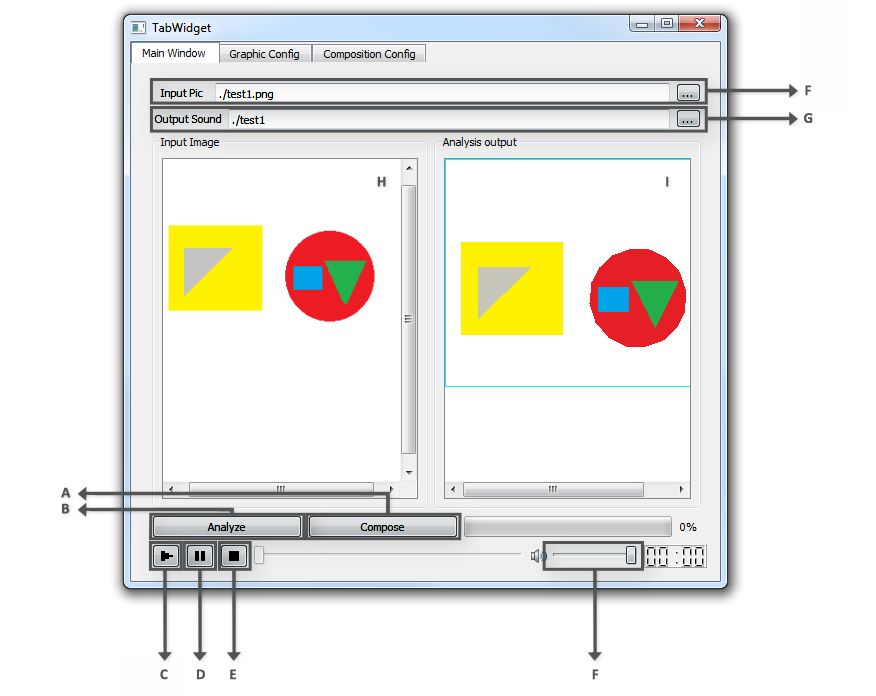
\includegraphics[scale=0.57]{graphics/interfaz.png}
		\caption{Vista general de la pestaña principal de la aplicación}
		\label{fig:interfaz}
		\end{figure}
		
		\noindent\textit{Carga de imagen de entrada [7]:}  Mediante esta opción el usuario puede elegir la dirección desde donde se cargará la imagen de entrada que se usará en el análisis. Para elegir la dirección podrá insertar el texto a mano o utilizar el botón para usar el explorador del sistema operativo correspondiente.\\
		
		\noindent\textit{Selección del archivo de audio de salida [8]:}  Mediante esta opción el usuario puede la dirección dodne se guardará el archivo de salida. Para elegir la dirección podrá insertar el texto a mano o utilizar el botón para usar el explorador del sistema operativo correspondiente.\\
		
		\noindent\textit{Input Image [A]:} En este panel se muestra la imagen elegida para el análisis.\\
		
		\noindent\textit{Analysis output [B]:} En este panel se muestra el resultado del último análisis realizado pulsando el botón "Analyze".\\
		
		\noindent\textit{Botón Analyze [2]:} Tal y como su nombre indica, Analyze, realiza el analisis de la imagen pasada como parámetro de entrada lanzando a ejecución el programa Phic, uno de los módulos de la aplicación. Tras analizarse, el resultado podrá observarse en el \textit{[B]}.\\
		
		\noindent\textit{Botón Compose [1]:} Realiza la composición musical a partir de los datos analizados, para ello lanza a ejecución el programa Mu, otro de los módulos de la aplicación. Una vez compuesta la pieza musical, se podrá escuchar mediante los controles de control de sonido.\\
		
		\noindent\textit{Botón de Inicio de Reproducción [3]:} Permite al usuario iniciar la reproducción de la pieza musical compuesta por el módulo Mu.\\
		
		\noindent\textit{Botón de Pausa de Reproducción [4]:} Pausa la pieza musical en reproducción.\\
		
		\noindent\textit{Botón de Detención de Reproducción [5]:} Detiene la reproducción completamente.\\
		
		\noindent\textit{Barra de sonido [6]:} Modifica el volumen de la reproducción en curso.

		
		\subsubsection{Configuración gráfica}
		
		En esta pestaña se encuentran todas las opciones relacionadas con el análisis de la imagen. En ella se podrán configurar opciones que hagan que el proceso de análisis varíe en velocidad, precisión o estilo.\\
		
		De entre los parámetros de configuración, existen los llamados ``generales'', que siempre aparecen visibles al usuario, y los ``específicos'', que complementan a los generales y sólo aparecen cuando el contexto lo especifica. En la Figura~\ref{fig:interfazgraphic} podemos ver detalladamente los parámetros generales.\\
		
		\begin{figure}[htbp]
		\centering
		\hspace*{-0.9in}
		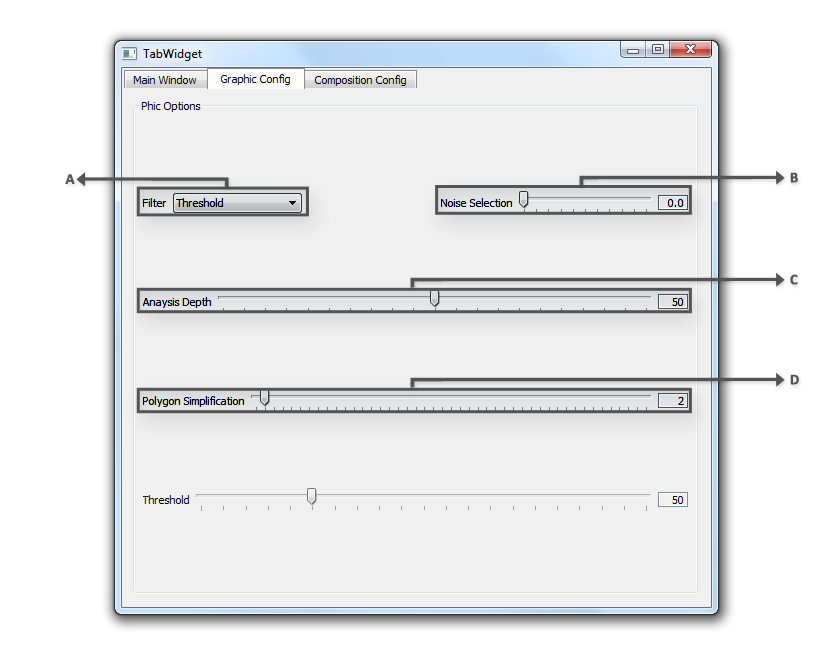
\includegraphics[scale=0.57]{graphics/interfazgraphic.png}
		\caption{Vista general de la pestaña de configuración gráfica}
		\label{fig:interfazgraphic}
		\end{figure}
		
		\noindent\textit{Tipo de filtrado de imagen [1]:} Distintos filtros en la imagen producirán diferentes formas de entender las formas que hay en ellas. De forma un poco más precisa, pero sin llegar a entrar en detalles técnicos, los filtros se encargan de transformar la imagen original a un mapa de bits en blanco y negro, que posteriormente se analizará para detectar polígonos en él. Un buen filtro diferenciará las deseadas superficies de color como manchas blancas independientes.\\
		
		\noindent\textit{Selección de ruido [2]:} Mediante esta barra el usuario puede elegir el tamaño mínimo de las formas por debajo del cual no se considerarán relevantes en el análisis. El valor representa un porcentaje respecto al area total de la imagen, de forma que un valor $n$ de Selección de Ruido determina que todas las formas con area menor a un $n$\% del area total de la imagen se considerarán ruido y no serán estudiadas.\\
		
		\noindent\textit{Profundidad del análisis [3]:} Permite variar el nivel de detalle con el que se realizará el análisis. Un valor de profundidad grande hará que el análisis se realice con gran parte los recursos que permite el programa (a costa de mayor lentitud en el análisis), mientras que un valores pequeños aumentarán la velocidad del proceso a costa de perder precisión a la hora de detectar formas de color.\\
		
		\noindent\textit{Simplificación de polígonos [4]:} Una vez detectadas las formas de color, es necesario aproximarlas a una lista de vértices para reducir el peso de la información sin modificar la carga de la misma. El nivel de fidelidad en la transformación de formas a polígonos se establece con este parámetro: un valor alto determina una gran fidelidad a costa de mayor tiempo de análisis, y viceversa.\\
		
		\noindent\textit{Botón Analyze [2]:} Tal y como su nombre indica, Analyze, realiza el analisis de la imagen pasada como parámetro de entrada lanzando a ejecución el programa Phic, uno de los módulos de la aplicación. Tras analizarse, el resultado podrá observarse en el \textit{[B]}.\\


		Los parámetros ``especícos'' dependen única y exclusivamente del tipo de filtro seleccionado [1], ya que cada tipo de filtro introduce nuevas opciones que configurar. \\
		
		
		Todo filtro en la aplicación que nos ocupa, como ya se comentó anteriormente, realizan la misma función: detectar formas y expresarlas como superficies blancas. A continuación se explica de forma general el funcionamiento de cada filtro y sus parámetros ``específicos''.\\
		
		
		\todo{HACER REFERENCIA A CADA ALGORTIMO QUE NO SEA NUESTRO (TODO MENOS HUE SELECTIONS Y MULTIPLE THRESHOLD) A LA DOC DE OPENCV O A ALGO}
		
	\noindent\textbf{Threshold}\\
		
		\begin{figure}[htbp]
		\centering
		\hspace*{-0.9in}
		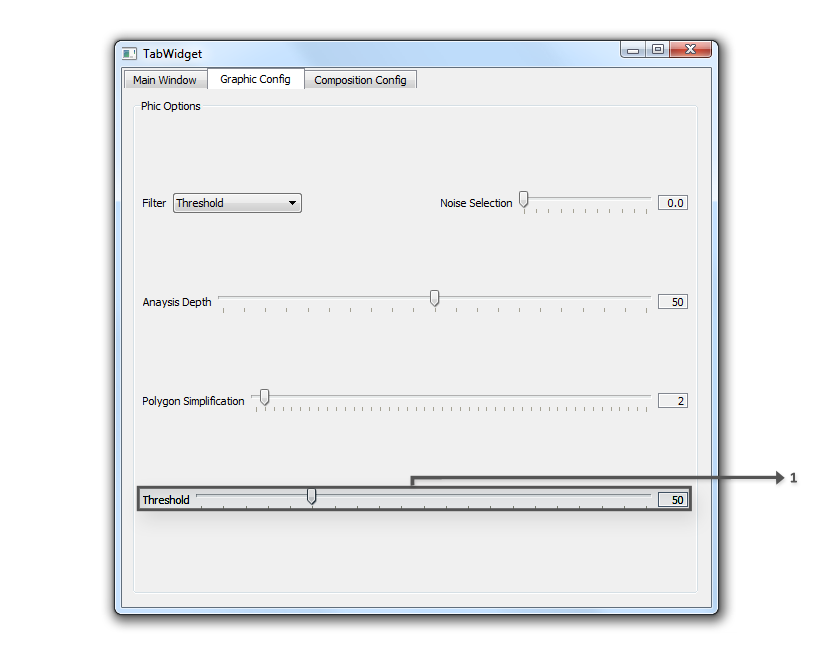
\includegraphics[scale=0.57]{graphics/interfazthreshold.png}
		\caption{Vista del filtro Threshold}
		\label{fig:interfazthreshold}
		\end{figure}
		
		Este filtro transforma la imagen a escala de grises para luego marcar como blancos todos los píxeles con un valor de gris superiores a un umbral dado, y como negros el resto.\\
		
		Los parámetros específicos que usa, vistos en la Figura~\ref{fig:interfazthreshold}, son:\\		
		
		\noindent\textit{Valor del umbral [1]:} Establece el valor del umbral antes explicado.\\
		
	\noindent\textbf{Adaptative Threshold}\\

		Mientras que el filtro anterior utiliza un mismo umbral para toda la imagen, Adaptative Threshold analiza cada parte de la imagen en escala de grises y decide qué umbral es mejor para cada sección.\\ 
		
		Este filtro no usa parámetros específicos, ya que recalcula el valor del umbral cada vez que le resulta necesario.\\
		
	\noindent\textbf{Canny}\\

		Utiliza el algoritmo de detección de regiones del mismo nombre, desarrollado en 1986 por John F. Canny. Una vez encontrados los bordes, establece las figuras que estos delimitan.\\
		
		Este filtro no usa parámetros específicos.\\
		
	\noindent\textbf{Hue Division}\\

		\begin{figure}[htbp]
		\centering
		\hspace*{-0.9in}
		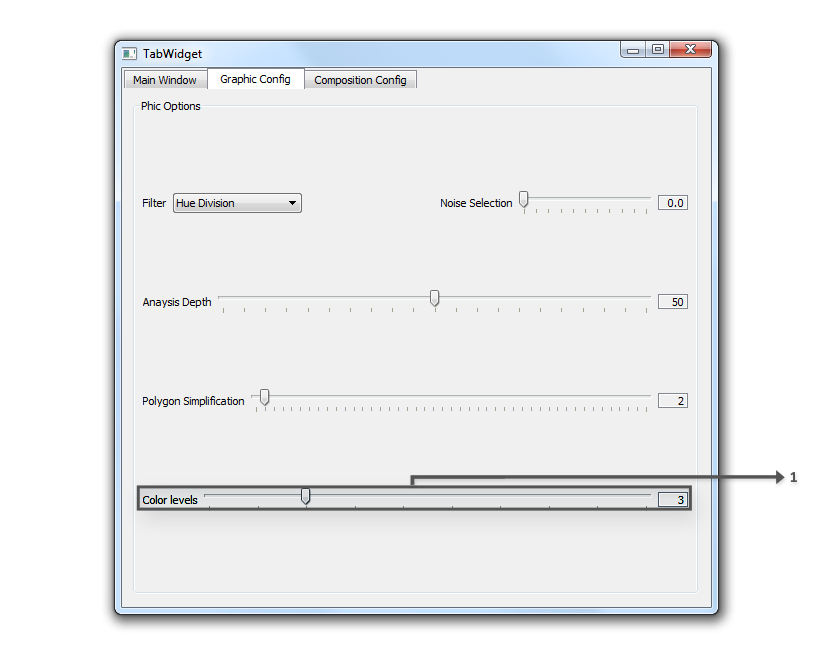
\includegraphics[scale=0.57]{graphics/interfazhue.png}
		\caption{Vista general del filtro Hue Division}
		\label{fig:interfazhue}
		\end{figure}

		Se trata de un filtro propio que busca asocia manchas de color con conjuntos de píxeles vecinos con valores RGB dentro de un mismo rango de rojo (R), azul (B) y verde (G). Los parámetros específicos son:\\
		
		\noindent\textit{Niveles de color[1]:} Este parámetro determina el número de intervalos posibles de color que puede haber en cada canal de color, y por tanto determinará la amplitud de cada rango. Un valor igual a 3 indica que un pixel cualquiera puede entrar dentro de 3 intervalos posibles en el canal rojo, otros 3 en el azul y otros 3 en el verde. De esta forma cada píxel entra dentro de una de las $3*3*3=27$ categorías de color, simplificando el análisis. Un valor muy grande de este parámetro hará que haya más categorías de color y que por tanto colores que antes se consideraban parte de una misma forma ahora se consideren como parte de formas independientes con colores más específicos. Un valor muy pequeño hará que se interpreten formas más amplias (incluyendo píxeles más diversos).\\
		
	\noindent\textbf{Color Threshold}\\

		\begin{figure}[htbp]
		\centering
		\hspace*{-0.9in}
		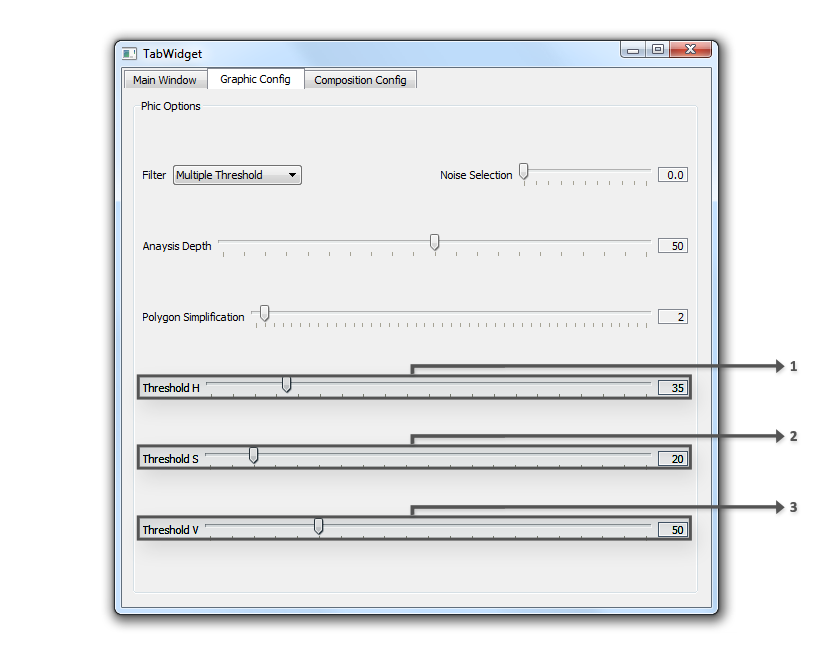
\includegraphics[scale=0.57]{graphics/interfaz3threshold.png}
		\caption{Vista general del filtro Color Threshold}
		\label{fig:interfaz3threshold}
		\end{figure}

		Se trata de un filtro propio que adapta el filtro Threshold para una imagen de 3 canales. En vez de considerar como figuras aquellas agrupaciones de píxeles cuyos valores en escala de grises sean inferiores a un umbral, considera aquellas que en su canal de Matiz (Hue), Saturación (Saturation) y Valor (Value) sean menor que un umbral, originando cada canal formas independientes.\\
		
		Los parámetros específicos de este filtro determinarán el valor de los umbrales de cada canal determinado en formato de imagen HSV.\\		
		
		\noindent\textit{Valor del umbral de Matiz[1]}\\
		\noindent\textit{Valor del umbral de Saturación[2]}\\
		\noindent\textit{Valor del umbral de Valor[3]}




		
		\subsubsection{Configuración de composición}
		
		Esta pestaña contiene todos los parámetros configurables relativos a la composición algoritmica. Estos, como muestra la Figura~\ref{fig:interfazcomp} son:\\
		
		\begin{figure}[htbp]
		\centering
		\hspace*{-0.9in}
		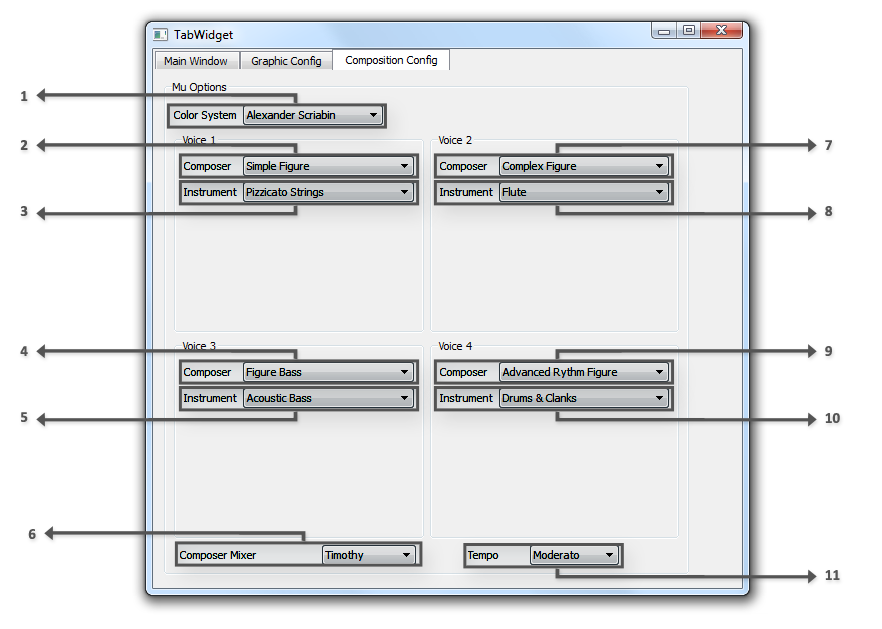
\includegraphics[scale=0.57]{graphics/interfazcomp.png}
		\caption{Vista general de la pestaña de configuración gráfica}
		\label{fig:interfazcomp}
		\end{figure}
		
		\noindent\textit{Sistema de color[1]:} Permite alternar entre las diferentes relaciones tono-color explicadas en el Capítulo~\ref{sec:algcomp}.\\
		
		\noindent\textit{Algoritmo de composición para la primera voz[2]:} Con esta opción, el usuario puede elegir, de entre los distintos algoritmos de composición, el que se usará para que generar la melodía principal.\\
		
		\noindent\textit{Algoritmo de composición para la segunda voz[7]:} Con esta opción, el usuario puede elegir, de entre los distintos algoritmos de composición, el que se usará para que generar la segunda melodía principal.\\

		\noindent\textit{Algoritmo de composición para la tercera voz[4]:} Con esta opción, el usuario puede elegir, de entre los distintos algoritmos de composición del bajo, el que se usará para que generar el bajo armónico.\\
		
		\noindent\textit{Algoritmo de composición para la cuarta voz[9]:} Con esta opción, el usuario puede elegir, de entre los distintos algoritmos de composición de ritmos, el que se usará para que generar el ritmo de la pieza musical final.\\
		
		\noindent\textit{Selección de instrumentos [3], [5], [8] y [10]:} Permiten seleccionar los instrumentos con los que sonaran las distintas voces.\\

		\noindent\textit{Algoritmo de composición general[6]:} Determina qué algoritmo se usará para recorrer la imagen y aplicar los algoritmos de las distintas voces. Se explica con detalle en el Capítulo~\ref{sec:algcomp}.\\

		\noindent\textit{Tempo[11]:} Como su nombre indica, su valor determina el tempo con el que sonará la pieza musical compuesta.\\
		
		
\section{Arquitectura}

\subsection{Formato de representación de música}

\todo{Repasar formalizar}

La estructura para representar la música propuesta en el proyecto está determinada por un árbol que trabaja desde el elemento más general, la canción que se va a componer, al más específico, cada una de las notas que componen dicha canción, como muestra la Figura~\ref{fig:structmusic}.\\
	
	\begin{figure}[htbp]
	\centering
	\hspace*{-0.67in}
	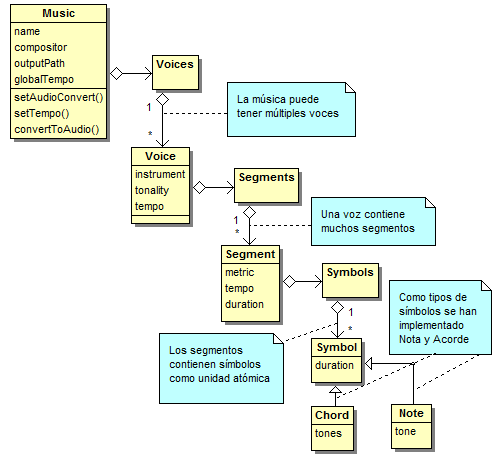
\includegraphics[scale=0.57]{graphics/musica-estructura.png}
	\caption{Estructura de la música}
	\label{fig:structmusic}
	\end{figure}


\textbf{Música}: Al nivel de la Música, trabajamos con la información relativa a toda la canción que se va a componer, por un lado está información relativa al nombre de la composición y del compositor que la ha hecho, también dispone de una serie de voces a partir de las cuales estará formada la canción y su tempo. Por último a un nivel más cercano, la implementación permitirá elegir con que herramienta querremos crear el archivo de audio de salida.
\newline

\textbf{Voz}: Por debajo de la Música se trabaja con las Voces. Su estructura permite determinar el instrumento, la tonalidad y el tempo de cada una de las voces que componen una Música, cada una de estas voces esta compuesta de varios segmentos musicales, los cuales al ser reproducidos en el orden establecido por el compositor forman la Voz en cuestión.
\newline

\textbf{Segmento}: Estos elementos tienen la posibilidad de establecer su propia métrica, su tempo y su duración. Los segmentos a su vez están formados por una sucesión de símbolos.
\newline

\textbf{Símbolo}: Son la unidad a partir de los cuales se crean todos los elementos básicos de la música, símbolo nos permite establecer una duración para estos elementos. Actualmente el proyecto crea dos tipos de elementos a partir de símbolo:
\begin{itemize}
\item \textbf{Notas}: Estos símbolos tienen asociada una duración, determinada por el componente anterior, y un tono establecido por un número que posteriormente será interpretado con la herramienta que generará el archivo de audio.
\item \textbf{Acordes}: Los acordes están formados de la misma manera que las notas pero en lugar de tener asociado un único tono pueden tener de dos a tres tonos diferentes, en la práctica esto resultará en todos los tonos sonando a la vez durante el mismo tiempo una vez generada la canción.
\end{itemize}

\subsection{Formato de representación de imágenes}

\todo{está en google docs, sólo es pasarlo a limpio}

\subsection{Sistema de análisis de Imágenes: Phic}

\todo{hacer}

\subsection{Sistema de composición algorítmica: Mu}

\todo{hacer}

\subsection{Sistema de enlace de módulos: Muphic}

\todo{hacer}

\subsubsection{Interfaz Gráfica}

El desarrollo de la interfáz gráfica se decidió realizar a través de un framework que facilitase la construcción de la misma. Qt, la herramienta que se utilizó se eligió debido a dos criterios, era multiplataforma, al igual que la aplicación, servía para trabajar con móviles, siguiendo así uno de los enfoques iniciales del proyecto que más adelante fue descartado. Además Qt trabaja con C++ como lenguaje de programación, el mismo que el núcleo de la aplicación y ofrece facilidades a la hora de integrar audio, a través de la librería Phonon, o componentes personalizados en una interfaz.\\
\todo{Este párrafo no se si abriría mejor la parte de arquitectura}
\newline
La interfáz esta compuesta de tres pestañas cada una encargada de una parte de la funcionalidad:
\newline
\\\underline{Graphic Config:}
\\En esta pestaña se encuentran todas las opciones relacionadas con el análisis de la imagen, las distintas configuraciones se transmitirán a los módulos de la aplicación a través de un documento XML que se genera cuando en la "Main Window" se le da al boton de "Analyze".
\\Los distintos componentes de esta pestaña van variando según el filtro que se seleccione, sin embargo algunos de ellos son comunes para todos los filtros:
\newline
\\\textit{Filter:} Este combo box permite seleccionar entre los distintos filtros que se pueden usar en la aplicación.
\\\textit{Noise Selection:} Con esta barra de desplazamiento se podrá elegir a partir de que tamaño, relativo al area del mayor polígono de la imagen, se ignorarán los poligonos encontrados durante el análisis de la imagen.
\\\textit{Analysis Depth:} Esta barra permite seleccionar cuanto deseamos comprimir la imagen original antes de analizarla, cuando menor sea su valor menor será el nivel de detalle obtenido y más rápido se realizará el análisis.
\\\textit{Polygon Simplification:} Esta barra permite seleccionar cuanto deseamos simplificar los poligonos obtenidos a partir de la imagen original, cuanto mayor sea su valor menos vertices tendrán los poligonos obtenidos y por lo tanto menos fiel será el resultado del análisis, sin embargo, este se realizará más rápido.
\newline
\\Según el filtro que se elija aparecerán mas componentes:
\newline
\\\todo{Rellenar esto de manera experta y didáctica}
\\\textit{Threshold} (Filtro Threshold): 
\\\textit{Hue Division} (Filtro Hue Division):
\\\textit{Threshold H} (Filtro Multiple Threshold):
\\\textit{Threshold S} (Filtro Multiple Threshold):
\\\textit{Threshold V} (Filtro Multiple Threshold):
\newline
\\\underline{Composition Config:}
\\En esta pestaña se pueden encontrar todas las opciones disponibles para el compositor musical, estás serán transmitidas a los modulos de la aplicacióncuando se pulse el boton de "Compose" en la "Main Window" a través del documento XML mencionado anteriormente.
\\Como se puede ver en la imagen adjunta, hay opciones para cuatro voces, que son aquellas con las que trabajan los compositores de la aplicación siendo, normalmente, la "Voice 1" la melodía principal, la "Voice 2" un acompañamiento, la "Voice 3" el bajo y la "Voice 4" la percusión. Las opciones disponibles son las siguientes:
\\\todo{Adjuntar imagen}
\newline
\\textit{Color System:} Hace referencia referencia a la teoría sinestésica que se utilizará como base para la relación de color-notas durante la composición musical.
\\textit{Composer:} En las cuatro voces se refiere a que compositor se utilizará para esa voz, al presionarlo se desplegarán los distintos compositores que estan disponibles para que el usuario elija el que mejor le convenga.
\\textit{Instrument:} En las cuatro voces se refiere a que instrumento se utilizará para esa voz en concreto, al presionarlo se desplegarán los instrumentos disponibles.
\\textit {Composer Mixer:} Hace referencia a que como se combinarán las cuatro voces anteriores.
\\textit{Tempo:} 
\\\todo{A rellenar con gente que sepa describirlo mejor que yo. \\También hay que repasar lo anterior}
\newline
\\{\bf Libreria Phonon}
\\Esta es una librería proporcionada por Qt para la reproducción de audio, al ser un módulo externo requiere una serie de librerias añadidas que están incluidas en el paquete de instalación de windows, sin embargo tendrán que ser instaladas en linux utilizando alguno de los gestores de software disponibles realizando una busqueda con la palabra clave: Phonon.
\\Las librerías requeridas son las siguientes: (LISTA DE LIBRERIAS)
\\En el caso de que no funcione el sistema de reproducción, se pueden encontrar los archivos de audio en la ruta especificada en "Midi Output"
\newline
\\\todo{Claramente esta parte va en arquitectura, sin embargo no se que más comentar de la arquitectura de la GUI puesto que casi todo esta hecho con QT, como no digamos el widget de carlos...}
\\La interacción con phonon se realiza utilizando la funcionalidad proporcionada por el framework. Se asocia el fichero multimedia a un tipo proporcionado por Phonon que a su vez lo conecta con el sistema de audio predeterminado para cada sistema operativo.
\\El uso de Phonon es conveniente porque a pesar de sus complicaciones ofrece una manera sencilla de incluir un reproductor en la interfaz, que a su vez, es multiplataforma sin obligar al usuario a buscar el archivo de audio o forzar una llamada a un tercer programa que reproducir la musica que generada.
\subsection{Futuras ampliaciones}
\chapter{Conclusiones}
\label{chap:results}

\gotrev{Última revisión realizada el 26-06-2012}

El objetivo inicial del proyecto era, como se ha detallado a lo largo del documento, construir una herramienta capaz de transmitir musicalmente lo que se percibe de una imagen. Tras 9 meses de proceso de desarrollo, se puede afirmar que se ha desarrollado de forma satisfactoria una aplicación capaz de llevar a cabo dicho objetivo, así como el resto de requisitos (tanto funcionales como no funcionales) mostrados en la Sección~\ref{sec:requisitos}.\\



Para llevar a cabo la aplicación, ésta se ha dividido en dos módulos independientes que trabajan de forma secuencial: el módulo de análisis de imagen en primer lugar, y el módulo encargado de la composición musical en segundo; los cuales se pueden asemejar a la etapa de estimulación visual y a la etapa de estimulación auditiva, respectivamente. Esta distinción ha dado la posibilidad de estudiar y probar las etapas de forma independiente y así poder experimentar las diferentes formas de abordar la interpretación música-imagen. Cabe destacar que, dado que esta relación debe ser objetiva y no dependiente de consideraciones culturales o personales (por especificación del sistema), se ha elegido la sinestesia como método de asociación entre la percepción visual y la auditiva.\\


Por un lado, el módulo de análisis ha resultado ser capaz de transformar cualquier tipo de imagen de entrada en una representación propia del sistema de forma suficientemente fiel en un espacio de tiempo corto (segundos): dada una correcta configuración de parámetros por parte del usuario, las imágenes de grandes dimensiones pueden ser tratadas con menos nivel de detalle para aumentar su velocidad. Además, se puede cambiar la manera de reconocer formas alternando entre los distintos algoritmos de análisis, permitiendo al usuario experimentar con la forma en la que quiere que una imagen sea captada. La correcta elaboración de este módulo ha sido una pieza clave para el desarrollo del proyecto ya que, aunque no sea el objetivo principal del mismo, proporciona la entrada al módulo de composición y por tanto una pieza clave para el perfecto funcionamiento de la generación de música.\\

Por otro lado, el módulo de composición ha cumplido con las expectativas mencionadas a lo largo del documento, siendo capaz de componer piezas musicales completamente originales que, si bien no buscan propiedades como ser ``pegadizas'', en ningún momento dejan de ser agradables al oído. Además, el módulo permite al usuario cambiar la forma de componer cada voz, así como los instrumentos con los que se interpretará cada una de ellas.\\

Con todo esto, la aplicación satisface la posibilidad de ser testeada por personas sinestésicas, de forma que éstas sean capaces de reconocer parcial o totalmente la similitud entre la imagen de entrada y la música generada. Con las diversas pruebas realizadas durante el desarrollo del proyecto, se ha determinado que la posibilidad de identificar la música creada a partir de las imágenes es factible, pero razonablemente limitada. Esto es debido a la cantidad de información que proporciona cada análisis de imagen, ya que sólo en las imágenes simples (con poca información) se puede anticipar la música generada. Por poner un ejemplo, una figura de cuatro vértices se asociará con cuatro notas. A cada figura interna dentro de ella se le asignará una melodía secundaría que sonará a la vez que la melodía de la figura padre. No hay que olvidar que, para añadir riqueza a la pieza musical, se añade una tercera voz (el bajo) y otra voz rítmica también basadas en las figuras presentes. Con todo esto, una figura de pocos vértices con unas pocas figuras dentro de ella tendrá asociada una pieza musical con cuatro voces tocando melodías distintas de una duración moderadamente corta a la vez. Por otro lado, una imagen analizada tiene del orden de un centenar de polígonos dentro de ella, cada uno de ellos con decenas de vértices. Puede imaginar el lector la complejidad que presentará la pieza musical generada, razón por la cual aumenta considerablemente la dificultad de comprender el origen de las notas que ha compuesto el algoritmo en cada momento.\\


\section{Usos de la aplicación}
\label{sec:usos}

Esta aplicación ha sido desarrollada teniendo en cuenta varios tipos de mercados (escenarios) y no sólo los pertenecientes al sector musical, ya que además de ellos se proponen otras alternativas. Es por ello que los usos para los cuales este sistema ha sido diseñado son:

\begin{itemize} 

\item\textbf{Ayuda a la composición:} Uno de los mayores problemas a la hora de componer es la búsqueda de inspiración para crear nuevas piezas musicales. Es por ello que un generador de música de esta índole, capaz de generar piezas originales y de un estilo razonablemente predecible (ya que depende de forma determinista de una imagen de entrada) es de gran utilidad en  este ámbito, siendo capaz de proporcionar ideas a los usuarios compositores. Con el objetivo de enfocar la aplicación a este aspecto, se ha establecido contacto con varios músicos quienes han mostrado su interés y admitido la posibilidad de usar la aplicación para tal fin. Durante sus experiencias, han preferido usar la aplicación con una gran variedad de imágenes, con la finalidad de abastecerse de piezas musicales variadas en lugar de intentar ver los diferentes efectos que puede tener el cambio de parámetros en una misma imagen, dado que el resultado sería una pieza musical similar a la pieza generada por primera vez. Sus opiniones han sido tremendamente positivas, apreciando la utilidad de dos aspectos de la aplicación: la creación de partituras, ya que sirve como base para componer una canción más complicada a partir de ella, y la reproducción de la música generada dentro del mismo entorno, gracias a la cual se puede comprobar rápidamente el resultado de una composición y se agiliza la realización de pruebas.

\item\textbf{Composición visual:} En una rama puramente artística, la asociación de imagen-música proporcionada por esta aplicación puede servir como punto de partida de una corriente artística que consista en elaborar piezas gráficas con la intención de ser interpretadas como música por ésta o una aplicación similar.


\item\textbf{Generación de música ambiente temática:} Como se ha establecido en la introducción de este documento, la generación musical desarrollada no pretende componer piezas musicales que sean capaces de ser el foco de atención del usuario durante su interpretación, sino que es su objetivo generar una música de ambiente capaz de sonar de fondo mientras el usuario realiza otra actividad. Dado que se une la percepción visual con la musical, es una forma más de realidad aumentada que puede servir como hilo musical de fondo en museos (con melodías asociadas a cuadros), anuncios (melodías asociadas al logo de la marca promocionada) o distintas situaciones cotidianas.

\item\textbf{Educación:} Tanto los niños pequeños como los discapacitados (con enfermedades como el autismo o similares) sienten una gran conexión con la música y están bastante atraídos por ella. Mediante el uso de esta aplicación pueden aprender a crear música de forma sencilla y además divertida, al mismo tiempo que entrena su percepción visual, desarrollando por tanto los dos sentidos simultáneamente. Se ha comentado esta idea a personas dentro del sector educativo que han mostrado interés en probar esta aplicación en cursos con alumnos más pequeños.

\end{itemize}

\section{Futuras ampliaciones}
\label{sec:ampliaciones}

Una vez desarrollada la aplicación, y siendo ésta completamente funcional, cabe plantearse las posibles ampliaciones que se podrían realizar sobre el sistema para incrementar su funcionalidad y usos. Muchas de ellas parten de la idea inicial del proyecto, con la intención de proporcionar robustez al sistema o mejorar su funcionalidad; otras buscan dar al sistema un nuevo enfoque de uso. Estas ampliaciones son:

\begin{itemize}

\item\textbf{Realización de nuevos y distintos algoritmos de composición:} Aunque los algoritmos desarrollados se basan todos en una idea común (la sinestesia), existen muchas maneras de interpretar una imagen estática como una pieza musical que evoluciona en el tiempo. El proyecto ha sido diseñado para poder añadir nuevos algoritmos
al código fuente de forma razonablemente sencilla. El proceso de desarrollo de estos algoritmos se basa intrínsecamente en el desarrollo y realización constante de pruebas, por lo que no existe una solución definitiva.\\

Para ello, se puede partir de ayuda externa para producir ideas (o bien búsqueda y lectura de investigaciones llevadas a cabo sobre estos aspectos de la composición, o bien contacto con compositores profesionales). Además, es necesaria en la elaboración de nuevos algoritmos un post-proceso de testeo de la cualidad de los mismos, ya que la calidad de las piezas musicales generadas por un algoritmo no se puede demostrar con completa seguridad hasta la finalización de la implementación de los algoritmos.

\item\textbf{Permitir la inclusión de nuevos algoritmos externos al código fuente.} Actualmente, la única manera de incluir nuevos algoritmos de composición o análisis es incluyéndolos en el código fuente de la aplicación. Una posible vía de desarrollo consistiría en dar la oportunidad al usuario de incluir nuevas formas de componer y analizar de forma externa, mediante nuevos módulos ejecutables o scripts que la aplicación sea capaz de lanzar.\\

\item\textbf{Expandir el formato de representación de imágenes}, de forma que sea capaz de almacenar más información sobre la imagen. La aplicación desarrollada sólo es capaz de representar internamente polígonos y sus posiciones y colores; pero hay mucha más información dentro de una imagen que nos puede ser útil:

	\begin{itemize}
	
		\item\textit{Reconocimiento de simetrías:} una imagen puede tener diferentes tipos de simetrías entre los objetos/colores que la forman. Información de este tipo puede servir de base a nuevos algoritmos de composición para que realicen melodías que repitan patrones o segmentos en función de las simetrías encontradas.
		
		\item\textit{Reconocimiento de composiciones:} no es poco común que las figuras de una imagen estén dispuestas siguiendo formas geométricas básicas (círculos o triángulos, por poner dos ejemplos). Un ejemplo bastante famoso se puede observar en la Figura~\ref{fig:composition}, donde se muestra la imagen de entrada a la izquierda y la composición que se pretende reconocer a la derecha. Imágenes con una disposición geométrica de figuras muy acentuada puede producir composiciones musicales cuya organización global sea equivalente a esta geometría detectada.\\
			
			\begin{figure}[!htbp]
			\centering
			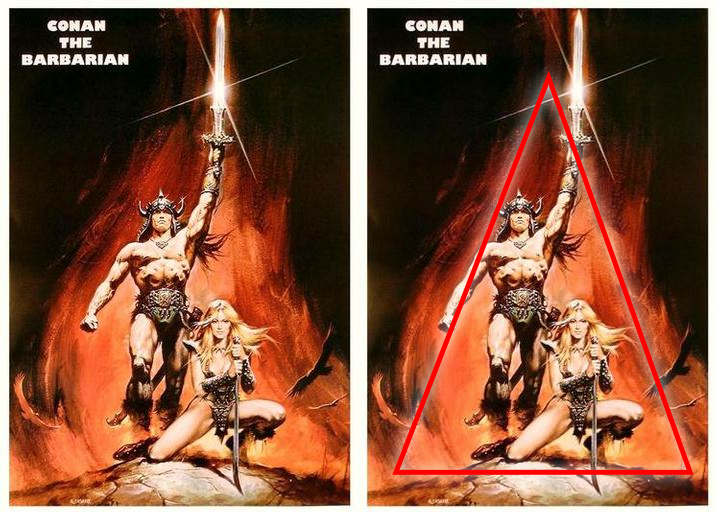
\includegraphics[scale=0.40]{graphics/composition2.png}
			\caption{Ejemplo de reconocimiento de una composición triangular.}
			\label{fig:composition}
			\end{figure}
		
		\item\textit{Reconocimiento de estructuras fractales:}
existen actualmente compositores algorítmicos que toman como entrada los parámetros de una estructura fractal para generar piezas musicales acordes a ella. De forma más ambiciosa, el proceso de análisis de este sistema podría distinguir aquellos casos en los que las figuras de una imagen forman entre sí estructuras fractales, es decir, donde formas básicas se repiten en diferentes dimensiones, como se da en la Figura~\ref{fig:fractal}. Posteriormente, esta información se pasaría a un compositor que tenga en cuenta estas estructuras.
		
			\begin{figure}[!htbp]
			\centering
			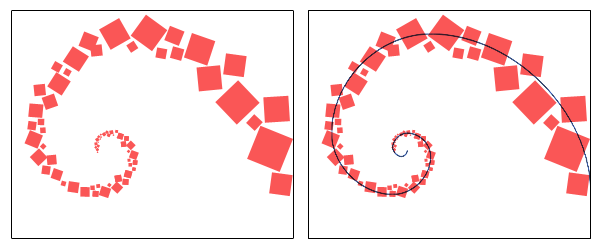
\includegraphics[scale=0.47]{graphics/fractal.png}
			\caption{Ejemplo de reconocimiento de una estructura fractal.}
			\label{fig:fractal}
			\end{figure}

		\item\textit{Ampliación de descripción del color de una figura:} la aplicación actual, con el objetivo de simplificar el proceso de análisis, sólo reconoce un color para cada figura reconocida. Sin embargo, la figura puede experimentar dentro de ella una variación de colores (aunque sea dentro de pequeños rangos), hecho que el sistema simplifica calculando el color medio. Esta ampliación consistiría en investigar una manera de detectar esa variación interna de color de forma que se consiga una representación más fiel de la figura.
	\end{itemize}
	
\item\textbf{Portar la aplicación a sistemas Apple.} Con esto se conseguiría expandir el número de posibles usuarios de la aplicación. Dado que las máquinas con sistema operativo de Apple funcionan con UNIX como base, esta ampliación puede resultar muy sencilla si se parte de la versión para Linux de la aplicación.

\item\textbf{Portar la aplicación a sistemas móviles.} Una de las ideas iniciales que se debatieron antes de comenzar el desarrollo de la aplicación fue la de implementar el sistema como una aplicación móvil. Sin embargo, al realizar el estudio de alcance del proyecto y el tiempo de desarrollo del mismo, se desechó la idea. Sin embargo, una aplicación de esta índole puede alcanzar un gran éxito en estos dispositivos ya que las cámaras integradas de los mismos proporcionan una entrada gráfica fácil y sencilla, lo cual sumado a la facilidad de uso del sistema, proporcionan a la aplicación un gran atractivo.\\ 

El sistema se ha diseñado para facilitar la implementación de dicha ampliación, eligiendo librerías disponibles tanto en sistemas operativos de ordenadores personales como de dispositivos móviles (ver Sección~\ref{chap:techs}).\\

\end{itemize}


\section{Seguimiento del proyecto}

La aplicación, para cada una de las plataformas que ha sido desarrollada, se puede descargar desde aquí:

\begin{center}
http://code.google.com/p/muphic/downloads/list
\end{center}

Algunas piezas musicales compuestas a partir de imágenes por el software desarrollado están disponibles en este canal de \emph{youtube}:

\begin{center}
http://www.youtube.com/user/mrmuphic
\end{center}

Con el tiempo se irán añadiendo más resultados de las diferentes composiciones relevantes o especiales que se vean convenientes.\\

Para contactar con el grupo de proyecto se puede hacer a través de la siguiente dirección:

\begin{center}
	imagebasedcomposing@gmail.com
\end{center}
\begin{thebibliography}{9}
\bibitem{portutesis}
  André Pintado Jorge Gonçalves,\\
  \emph{$Sense^{2}$ A Music System based on Paintings}.\\
  Dissertação para obtenção do Grau de Mestre em Engenharia Informática e de Computadores,\\
  Octubre 2009.
 \url{https://dspace.ist.utl.pt/bitstream/2295/570110/1/dissertacao.pdf}

\bibitem{paperSyn}
  V.S. Ramachandran \& E.M. Hubbard,\\
  \emph{Synaesthesia - A Window Into Perception, Thought and Language},\\
  Journal of Conscousness Studies, 8, 3-34,\\
  2001.

 \bibitem{colorpsy}
  Andrew J. Elliot (University of Rochester), Markus A. Maier (University of Munich), Arlen C. Moller and Ron Friedman (University of Rochester), and Jörg Meinhardt (Univeristy of Munich)\\
  \emph{Color and Psychological Functioning: The Effect of Red on Performance Attainment},\\
  Febrery 2007.  

 \bibitem{BrianEnoInterview}
  \emph{Brian Eno's Thoughts On Ambient Music},\\
  Interview at Synthtopia,\\
  \url{http://www.synthtopia.com/content/2009/09/17/brian-enos-thoughts-on-ambient-music/}

 \bibitem{opencvDoc}
  \emph{OpenCV 2.1 C++ Reference},\\
  \url{http://opencv.willowgarage.com/documentation/cpp/index.html}

 \bibitem{qtlibs}
  \emph{Librerías Qt versión 4.7.4},\\
  \url{http://qt.nokia.com/downloads}

\bibitem{organosColor}
 William Moritz
 \emph{The Dream of Color Music, and Machines that made it possible},\\
 Animation World, Issue 2.1, April 1997,\\ 
 \url{http://www.awn.com/mag/issue2.1/articles/moritz2.1.html}

\bibitem{AIMethodsForComposition}
 G. Papadopoulos and G. Wiggins,
 \emph{AI Methods for Algorithmic Composition: A Survey, a Critical View  and Future Prospect},\\
 Proceedings of the AISB’99 Symposium on Musical Creativity\\
 Edinburgh, UK, 1999.\\
 \url{http://qmul.academia.edu/GeraintWiggins/Papers/201960/AI_Methods_for_Algorithmic_Composition_A_Survey_a_Critical_View_and_Future_Prospects}

\bibitem{AIMusicSurvey}
 Arshia Cont,
 \emph{Artificial Intelligence and Music: A critical survey and proposal},\\
 May 2005, University of California at San Diego.\\
 \url{http://cosmal.ucsd.edu/arshia/papers/AI_Music_survey.pdf}

\bibitem{HistoryAlgorithmicComp}
 Jhon A. Maurer,
 \emph{A Brief History of Algorithmic Composition},\\
 March, 1999.
 \url{https://ccrma.stanford.edu/~blackrse/algorithm.html}

\bibitem{SICOM}
 F. Pereira, C. Grilo, L. Macedo, and A. Cardoso,
 \emph{Composing Music with Case-Based Reasoning}
 International Conference on Computational Models of Creative Cognition, Dublin, 1997.
 \url{http://iconline.ipleiria.pt/bitstream/10400.8/94/1/ICCMCC1997.pdf}

\bibitem{GenJam}
 John Biles,
 \emph{GenJam: A Genetic Algorithm for Generating Jazz Solos},\\
 1994.\\
 \url{http://citeseerx.ist.psu.edu/viewdoc/summary?doi=10.1.1.55.6146}

\bibitem{AudioVisualSurvey}
 K. Giannakis and M. Smith,
 \emph{Imaging Soundscapes: Identifying Cognitive Associations between Auditory and Visual Dimensions},\\
 Godoy, R. I., Jorgensen, H. (eds.): Musical Imagery, Swets \& Zeitlinger, pp. 161-179, 2001.\\
 \url{http://quod.lib.umich.edu/cgi/p/pod/dod-idx?c=icmc;idno=bbp2372.2000.167}

\bibitem{Phonogramme}
 V. Lesbros,
 \emph{From Images to Sounds: A Dual Representation},\\
 Computer Music Journal 20 (3), pp. 59-69, 1996.\\
 \url{http://www.jstor.org/discover/10.2307/3680824?uid=3737952&uid=2129&uid=2&uid=70&uid=4&sid=56229244313}

\bibitem{bricksConvertsMusic}
 Dimitrios Margounakis, Dionysios Politis,
 \emph{Converting Images to Music using their Colour Properties},\\ 
 Proceedings of the 12th International Conference on Auditory Display, London, UK, June 20-23, 2006.\\
 \url{http://www.dcs.qmul.ac.uk/research/imc/icad2006/proceedings/papers/f66.pdf}

\bibitem{ImageBaseComposition}
 Xiaoying Wu, Ze-Nian Li,
 \emph{A Study of Image-based Music Composition}
 Multimedia and Expo, 2008 IEEE International Conference on. (pp. 1345-1348)\\
 Hannover, June 23 2008-April 26 2008.\\
 \url{https://www.cs.sfu.ca/research/groups/VML/image_based_music/wu_icme08.pdf}

\bibitem{micrologus}
 Guido d'Arezzo,
 \emph{Micrologus},
 1027,
 traducido al inglés por Warren Babb.

\bibitem{VideoRedesFliparColores}
 David Eagleman,
 \emph{Redes: Flipar en Colores},\\
 Emisión Redes cap 22, 9 Febrero 2009.\\
 \url{http://www.redesparalaciencia.com/249/redes/redes-22-flipar-en-colores-29-minutos}

\bibitem{DeSensuEtSensato}
 Aristóteles,
 \emph{De Sensu et Sensato}

\bibitem{OpticksNewton}
 Isaac Newton,
 \emph{Opticks}

\bibitem{ScriabinQuintasColor}
 Ingrid Calvo Ivanovic,
 \emph{Sinestesia Cromática}
 \url{http://www.proyectacolor.cl/significados-del-color/sinestesia-cromatica/}

\bibitem{ConcerningSpiritualArt}
 Wassily Wassilyevich Kandinsky,
 \emph{Concerning the Spiritual in Art},\\
 1911.

\bibitem{GestaltPsychology}
 Wolfgang Köhler,
 \emph{Gestalt Psychology},\\
 Nueva York: Liveright. (1929).

 \bibitem{phononQt}
 Nokia Corporation
 \emph{Qt Development Network: Phonon Module}
 \url{http://qt-project.org/doc/qt-4.8/phonon-module.html}
 
 \bibitem{phononOverview}
 Nokia Corporation
 \emph{Qt Development Network: Phonon Overview}
 \url{http://doc.trolltech.com/4.4/phonon-overview.html}

\bibitem{TheUnityOfTheSenses}
 Lawrence E. Marks,
 \emph{The Unity Of The Senses},\\
 1978, 93.

\bibitem{pajares}
 Gonzalo Pajares, Jesús M. de la Cruz,\\
 \emph{Visión por Computador: Imágenes digitales y aplicaciones}\\
 RA-MA,\\
 2001.

\end{thebibliography}

\end{document}